\documentclass[a4paper,11pt]{article}

% --- Packages ---
% Language
\usepackage[utf8]{inputenc}
\usepackage[T1]{fontenc}
\usepackage[english]{babel}
% Font
\usepackage{lmodern}
\usepackage{graphicx}

% Math
\usepackage{amsmath,amssymb,amsfonts,mathrsfs}
\usepackage[amsmath,thmmarks]{ntheorem}

\usepackage{fancyhdr}
\usepackage{lastpage}
\usepackage{float}
%Commands
\renewcommand{\labelenumi}{(\alph{enumi})}
\renewcommand{\labelenumii}{(\arabic{enumii})}

\usepackage{algorithm2e}

% --- Definitions ---
% Counter
\newcounter{behctr}
% Math-German work
\newtheorem{claim}[behctr]{Claim}
\newtheorem{rmk}{Remark}
%% Proof environment with a small square as a "qed" symbol
\theoremstyle{nonumberplain}
\newtheorem{defn}{Definition}
\newtheorem{thm}{Theorem}
%\theoremheaderfont{\normalfont\slshape}
\theorembodyfont{\normalfont}
\theoremsymbol{\ensuremath{\square}}
\newtheorem{proof}{Proof}
\setlength\theorempostskipamount{0pt}
\setlength\theorempreskipamount{5pt}
% Math-commands
\newcommand{\inv}{^{-1}}
\newcommand{\vnorm}[1]{\left|\left|#1\right|\right|}
\newcommand{\set}[2]{\{\nonscript\,{#1}\mid{#2}\nonscript\,\}}
\DeclareMathOperator{\dist}{dist}
\DeclareMathOperator{\di}{d}
\DeclareMathOperator{\prio}{prio}
\DeclareMathOperator{\Root}{root}
\DeclareMathOperator{\rank}{rk}
\DeclareMathOperator{\key}{key}
\DeclareMathOperator{\vbl}{vbl}
\DeclareMathOperator{\id}{id}
\DeclareMathOperator{\CH}{CH}
\DeclareMathOperator{\Inv}{Inv}
\DeclareMathOperator{\Aut}{Aut}
\DeclareMathOperator{\Ker}{Ker}
\DeclareMathOperator{\Image}{Im}
\DeclareMathOperator{\supp}{supp}
\DeclareMathOperator{\grad}{grad}
\DeclareMathOperator\nN{\mathbb{N}}
\DeclareMathOperator\nZ{\mathbb{Z}}
\DeclareMathOperator\nQ{\mathbb{Q}}
\DeclareMathOperator\nR{\mathbb{R}}
\DeclareMathOperator\nC{\mathbb{C}}
\DeclareMathOperator\nH{\mathbb{H}}
\DeclareMathOperator\nD{\mathbb{D}}
\let\oldhat\hat
\renewcommand{\vec}[1]{\mathbf{#1}}
\renewcommand{\hat}[1]{\oldhat{\mathbf{#1}}}
\everymath{\displaystyle\everymath{}}

% --- Layout ---
\pagestyle{fancy}

% Text
\addtolength{\textwidth}{2cm}
\addtolength{\oddsidemargin}{-1cm}
\addtolength{\evensidemargin}{-1cm}
\addtolength{\textheight}{1.5cm}
\addtolength{\headheight}{2pt}
\addtolength{\topmargin}{-0.5cm}
\addtolength{\headsep}{-0.25cm}
% Footer
\renewcommand{\footrulewidth}{0.4pt}
\fancyfootoffset{-4cm}
\lfoot{}
\cfoot{\thepage\ / \pageref{LastPage}}
\rfoot{}
\title{\textbf{DD2427 - Exercise Set 8\bigskip}}
\author{Bertrand Mermet}
\date{}


% -----------------------
% ///--- Document --- \\\
% -----------------------

\begin{document}
\maketitle

\section{Exercise 1}
\subsection{Question 1}
\begin{figure}[H]
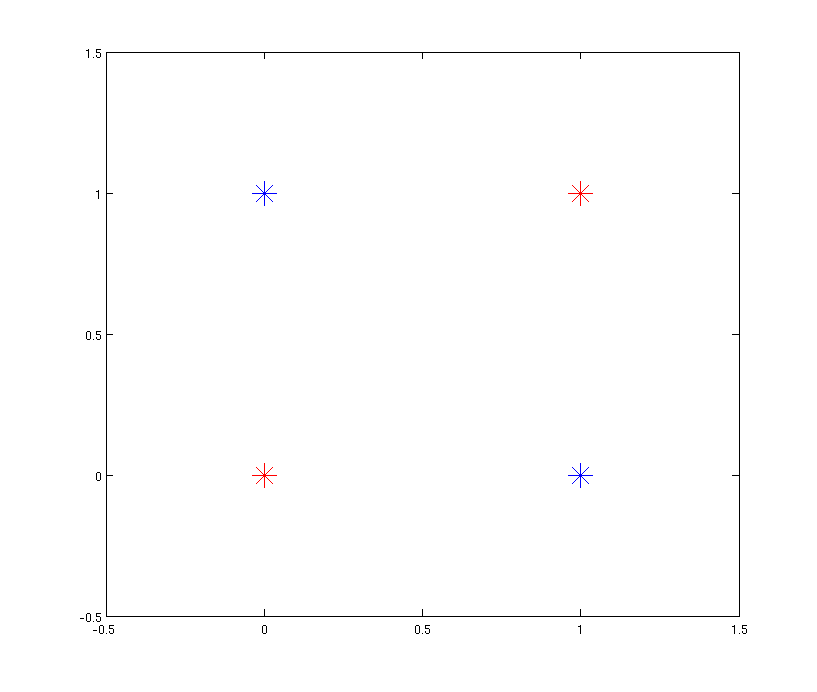
\includegraphics[width=100mm]{xor.png}
\end{figure}
The points are not linearly separable. The figure shows clearly that it is not possible to separe the red points from the blue one with a line.
\subsection{Question 2}
Let's apply one step of the boosting algorithm with vertical and horizontal lines.
\begin{itemize}
    \item We initialize the weights $D_i^1 = \frac{1}{4}$.
    \item We choose a vertical or an horizontal separation line (we call $h_1$ the so defined classifier).
    \item We compute the error and the strong classifier weight:
        \[
            \epsilon_1 = \sum^4_i{D_i^1 \cdot Ind(y_i \not= h_1(x_i))} = \frac{1}{2} 
        \]
        Because any line we can choose will misclassify half of the samples
        \[
            \alpha{1} = \frac{1}{2}\ln{\frac{1 - \epsilon_1}{\epsilon_1}} = 0
        \]
    \item We update the data weights:
        \[
        D_i^2 = \frac{D_i^1 exp(-\alpha_1y_1h_1(x_i))}{Z_1} = \frac{1}{4} 
    \]
\end{itemize}
Since all vertical and horizontal lines will have a weight of 0 in the strong classifier, it is impossible to solve the xor problem in this way.



\end{document}
